The User Interface design was developed based on the feedback and guidelines set by the clients, the Biology department staff. As it was an abstraction, we decided developing it in Microsoft Power Point was adequate for flexibility of the deisgn document and provides sufficient tools to make it presentable. Four main stages of the UI were separated into five slides which are provided and explained below.


\subsubsection{Sequence entry}
The first slide shows the sequence entry screen, where the user copies the DNA sequence on which to perform PCR into the provided box. The backward DNA strand is calculated right away and shown in green text, with each line being a complementary sequence of the one above. The numbers on the left show the node number at the start of the corresponding line. It is a way for the user to quickly find the part of the sequence to be amplified in the next stage and to provide better orientation in the sequence altogether. Scrolling through the sequence is done by pressing the arrow buttons on the right or just using the scroll wheel of the mouse. Once the user is content with the sequence entered, he can press the "Go" button to advance to the next stage.

\begin{figure}[h]
  \begin{center}
	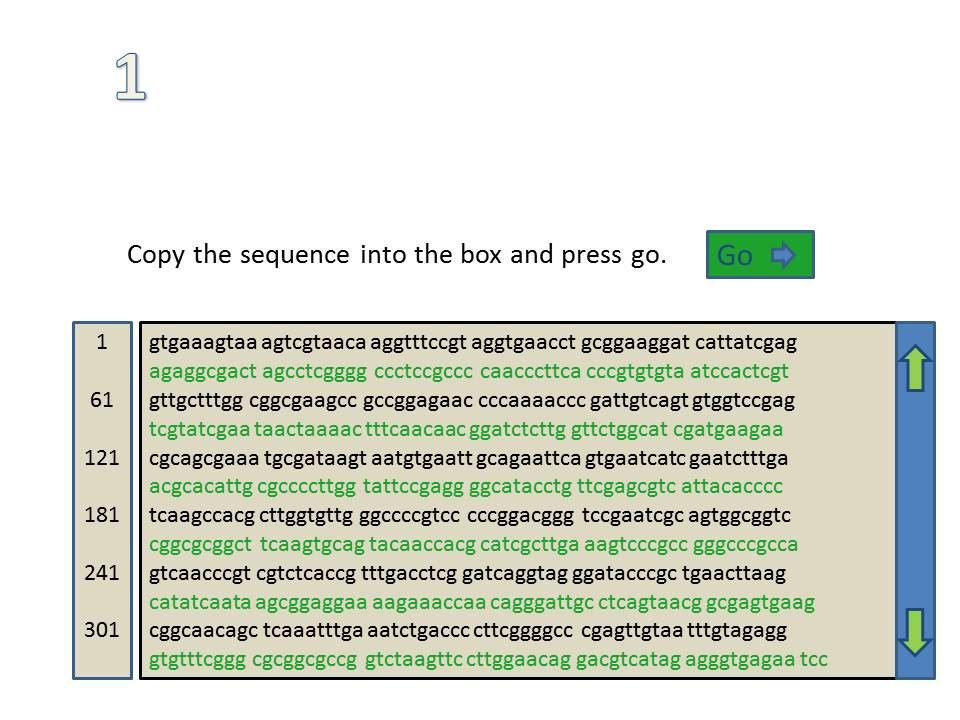
\includegraphics[width=0.6\textwidth]{./images/UiDes/Slide1.JPG}
    \caption{
      \label{fig:UiDes:slide1}
      Initial design, Sequence entry
    }
  \end{center}
\end{figure}

\subsubsection{Specification of target area}
The second slide shows the selection of the DNA sequence part to be amplified by PCR. The user enters the first and the final node numbers in the boxes "From" and "To" respectively, and the chosen area is highlighted after the user presses the "Enter" button. All of the previously introduced functions of the UI, including DNA sequence editing, are present at this stage also. When the user is content with the area specified, he can press the "Go" button to advance to the next stage. The "Go" button color is changed to clearly differentiate from the "Enter" button.

\begin{figure}[h]
  \begin{center}
	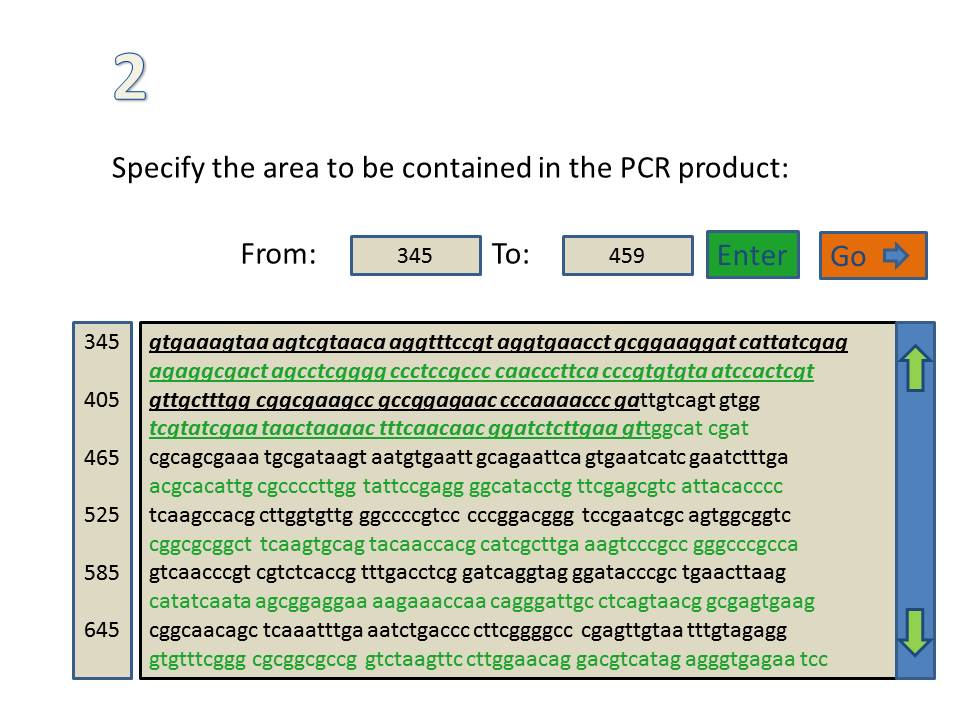
\includegraphics[width=0.6\textwidth]{./images/UiDes/Slide2.JPG}
    \caption{
      \label{fig:UiDes:slide2}
      Initial design,Specification of target area
    }
  \end{center}
\end{figure}

\subsubsection{Primer selection}
Primer selection UI stage is in our view the most important as it is the central part of the exercise, so it is explained extensively by the design document. User is required to copy or type the forward and the backward primers into the boxes above the sequence. The rules of primer design can be viewed by pressing the "Rules" button. If the user decides to change the target area or the sequence itself, he can go back to the previous stage by pressing the "Back" button. 

\begin{figure}[h]
  \begin{center}
	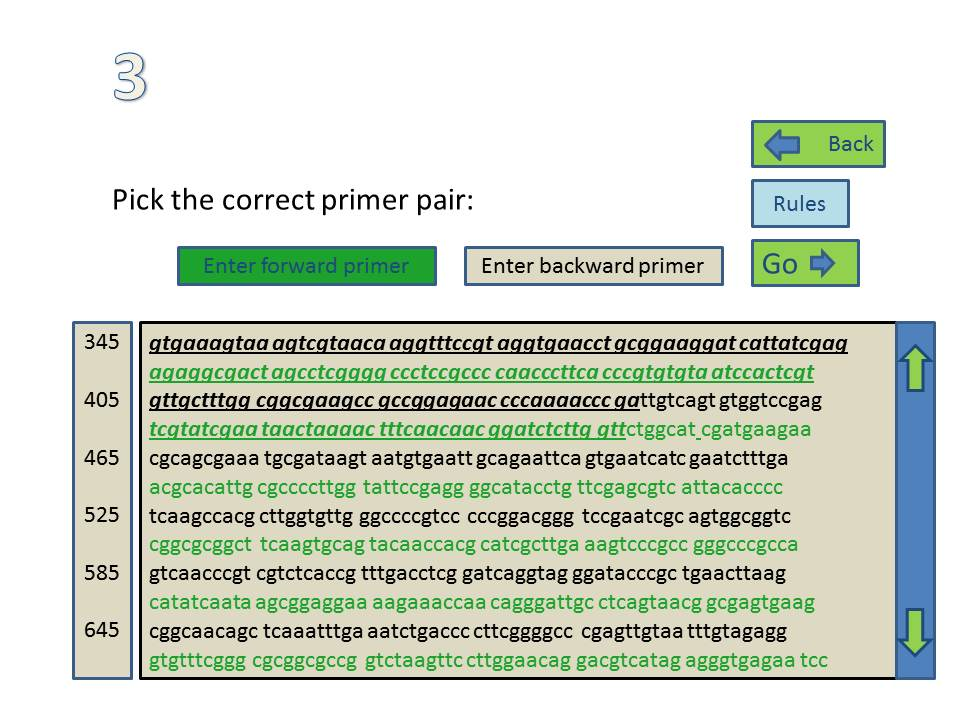
\includegraphics[width=0.6\textwidth]{./images/UiDes/slide3.jpg}
    \caption{
      \label{fig:UiDes:slide3}
      Initial design, Primer selection - initial screen
    }
  \end{center}
\end{figure}



When the user has entered the primers into their respective boxes, like shown below, he can press the "Go" button to go to the next stage if the primers are correct, or be shown an error message if they aren't.

\begin{figure}[h]
  \begin{center}
	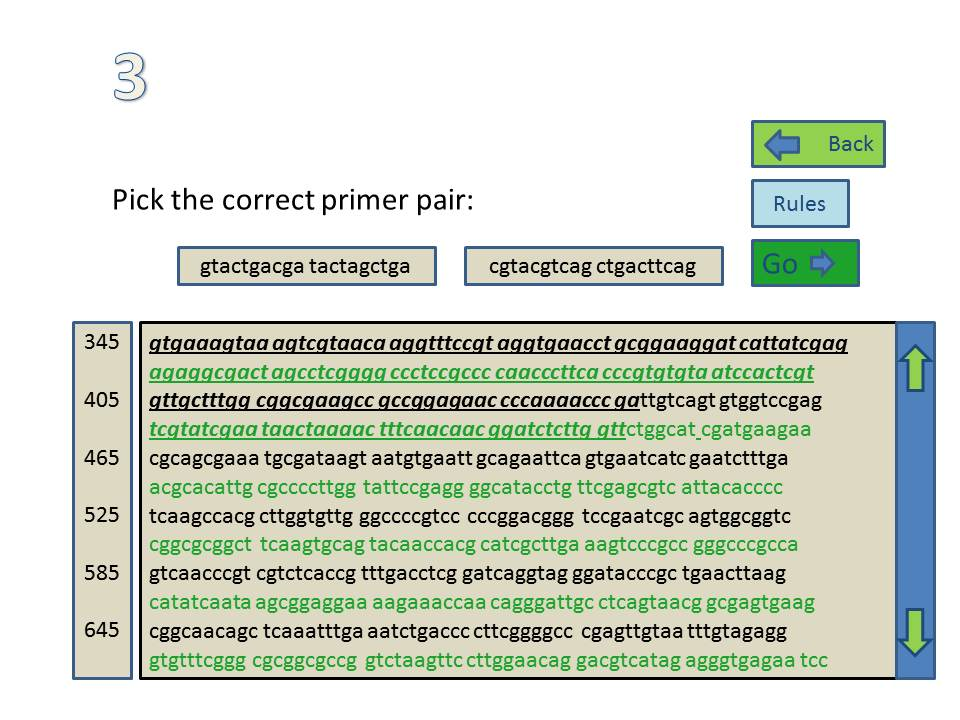
\includegraphics[width=0.6\textwidth]{./images/UiDes/Slide4.JPG}
    \caption{
      \label{fig:UiDes:slide4}
      Initial design, Primer selection - primers entered
    }
  \end{center}
\end{figure}

Each primer is checked for correctness according to the primer design rules and the user is shown a message explaining why his chosen primer is incorrect for the target sequence. In case both primers are incorrect, a separate list of errors is shown for each one. The user can then press the white arrow button to go back to selecting the primers.

\begin{figure}[h]
  \begin{center}
	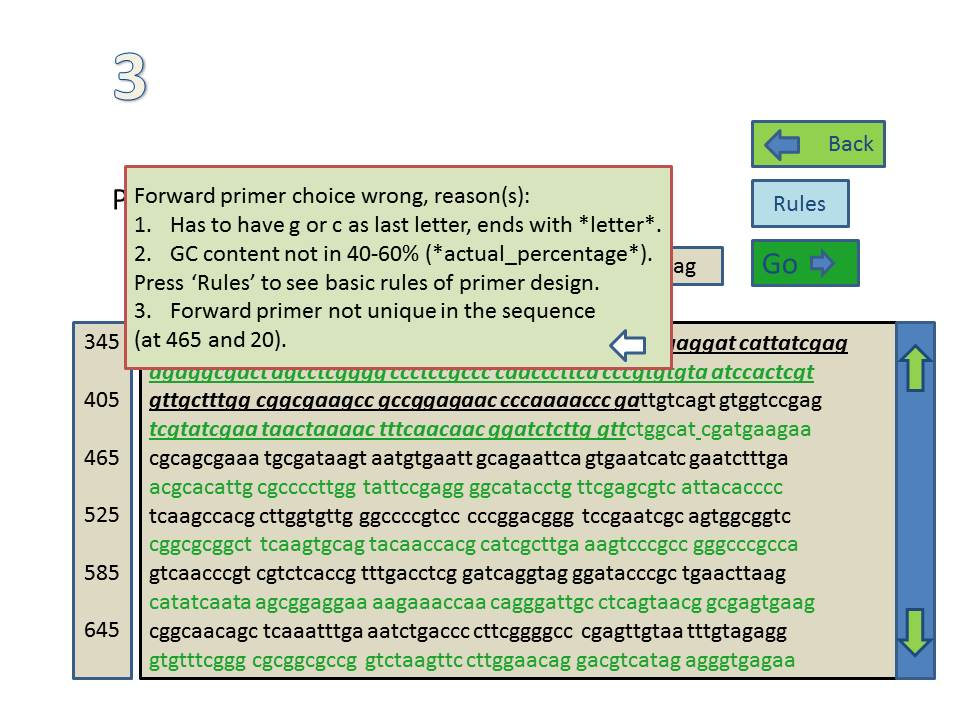
\includegraphics[width=0.6\textwidth]{./images/UiDes/slide5.jpg}
    \caption{
      \label{fig:UiDes:slide5}
      Initial design, Primer selection - error message
    }
  \end{center}
\end{figure}

\subsubsection{Melting temperature check}
The last slide shows the primers chosen by the user still in their respective boxes and their melting temperatures just below. Both temperatures must be in the range of 50 to 60 degrees Celsium for PCR to work, so if they aren't the user is suggested going back to the previous screen and selecting a different primer pair. As before, pressing "Back" will take the user to a previous stage. The user is also advised to visit the NCBI website (\cite{ncbi}) and performing primer blast on his selected primers to check them for specificity. Lastly, pressing the "Go" button will open a new window with an animation of PCR in action.

\begin{figure}[h]
  \begin{center}
	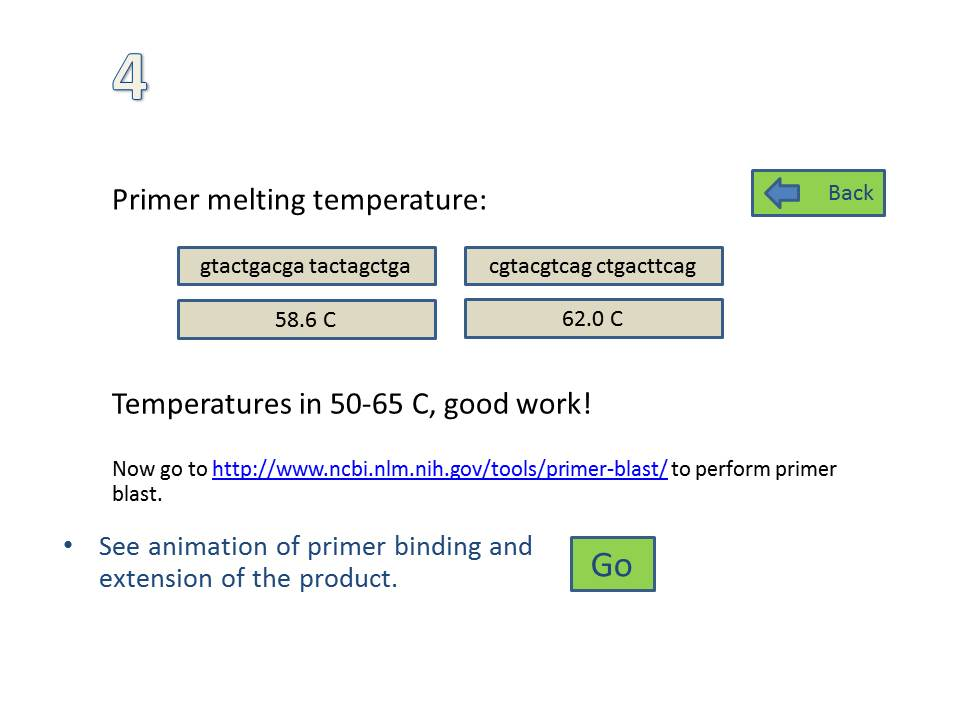
\includegraphics[width=0.6\textwidth]{./images/UiDes/Slide6.JPG}
    \caption{
      \label{fig:UiDes:slide6}
      Initial design, Primer melting temperatures
    }
  \end{center}
\end{figure}

